\documentclass[11pt]{article}

\usepackage{amsmath, amssymb, amsthm}
\usepackage{tikz}

\theoremstyle{plain}
\newtheorem{thm}{Theorem}[section]
\newtheorem*{thm*}{Theorem}
\newtheorem{prop}[thm]{Proposition}
\newtheorem{lem}[thm]{Lemma}
\newtheorem*{lem*}{Lemma}
\newtheorem{dfn}[thm]{Definition}
\newtheorem{cor}[thm]{Corollary}
\newtheorem{claim}[thm]{Claim}
\newtheorem{conj}[thm]{Conjecture}
\newtheorem{ques}[thm]{Question}
\newtheorem*{rem}{Remark}


\oddsidemargin  0pt
\evensidemargin 0pt
\marginparwidth 40pt
\marginparsep 10pt
\topmargin 0pt
\headsep 10pt
\textheight 8.2in
\textwidth 6.4in
\renewcommand{\baselinestretch}{1.1}

\newcommand{\codeg}{\text{codeg}}
\newcommand{\BBE}{\mathbb{E}}
\newcommand{\BFP}{\mathbf{P}}
\usepackage{amsmath}
\usepackage{amsthm}
\usepackage{amssymb}
\usepackage{mathtools}
\usepackage{hyperref}
\usepackage{url}





\usepackage{graphicx}
\usepackage{caption}
\usepackage{subcaption}

\def\eQb#1\eQe{\begin{eqnarray*}#1\end{eqnarray*}}
\def\eQnb#1\eQne{\begin{eqnarray}#1\end{eqnarray}}
\providecommand{\e}[1]{\ensuremath{\times 10^{#1}}}
\providecommand{\pb}[0]{\pagebreak}
\DeclarePairedDelimiter\ceil{\lceil}{\rceil}
\DeclarePairedDelimiter\floor{\lfloor}{\rfloor}

\newcommand{\E}{\mathrm{E}}
\newcommand{\Var}{\mathrm{Var}}
\newcommand{\Cov}{\mathrm{Cov}}

\def\Qb#1\Qe{\begin{question}#1\end{question}}
\def\Sb#1\Se{\begin{solution}#1\end{solution}}


\newtheoremstyle{quest}{\topsep}{\topsep}{}{}{\bfseries}{}{ }{\thmname{#1}\thmnote{ #3}.}
\theoremstyle{quest}
\newtheorem*{definition}{Definition}
\newtheorem*{theorem}{Theorem}
\newtheorem*{lemma}{Lemma}
\newtheorem*{question}{Question}
\newtheorem*{preposition}{Preposition}
\newtheorem*{exercise}{Exercise}
\newtheorem*{challengeproblem}{Challenge Problem}
\newtheorem*{solution}{Solution}
\newtheorem*{remark}{Remark}
\usepackage{verbatimbox}
\usepackage{listings}
\usepackage{mathrsfs}
\date{}
\title{\vspace{-0.7cm}
PDE II: Problem Set II}

\author{
Youngduck Choi 
\thanks{Department of Mathematics, Courant Institute of Mathematical Sciences, 
yc1104@nyu.edu; If you find an error and want to share with me, 
you can reach me via email.
}}

\begin{document}

\maketitle

\begin{abstract}
This work contains solutions for the problem set II.
\end{abstract}


\begin{question}[1-1]
\hfill
\begin{figure}[h!]
  \centering
    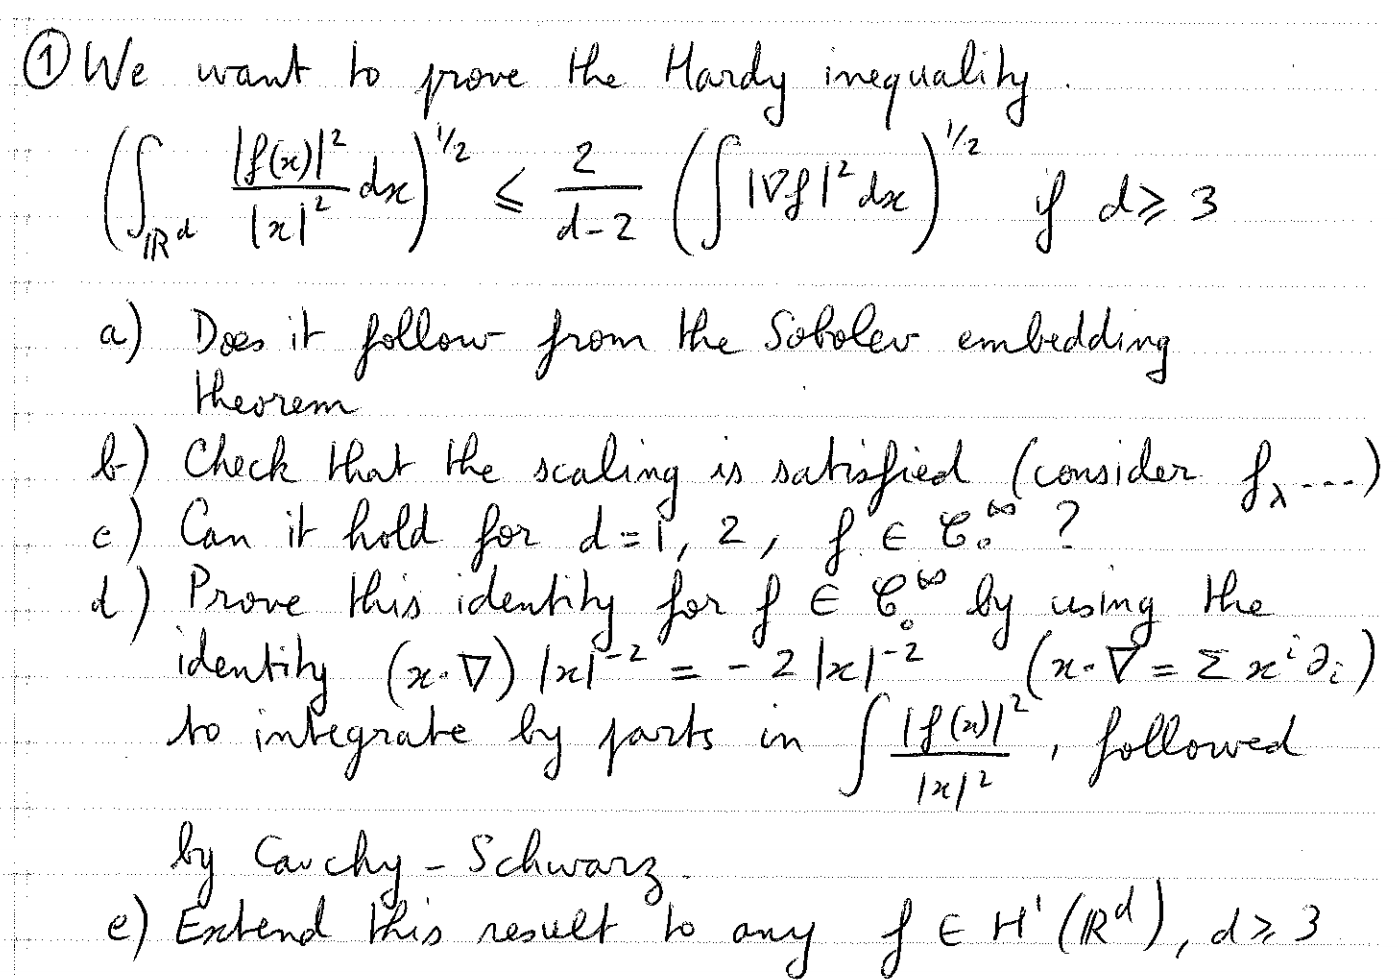
\includegraphics[width=0.7\textwidth]{pde2-s34-p1.png}
\end{figure}
\end{question}
\begin{solution} \hfill \\
\textbf{(a)} It does not follow from sobolev embedding, as $||\cdot||_{H^1(
\mathbb{R}^d)}$ is not equivalent to $||\triangledown \cdot ||_{L^2(\mathbb{R}_d)}$. 

\bigskip

\noindent \textbf{(b)} Let $f$ satisfy the inequality. Then, by a change of variables,
\eQb
\left( \int_{\mathbb{R}^d} \dfrac{|f(\lambda x)|^2}{|x|^2} dx \right)^{\frac{1}{2}}
&=& |\lambda|^{\frac{2-d}{2}} 
\left( \int_{\mathbb{R}^d} \dfrac{|f(x)|^2}{|x|^2} dx \right)^{\frac{1}{2}} \\ 
&\leq& \dfrac{2}{d-2} |\lambda|^{\frac{2-d}{2}} \left(\int_{\mathbb{R^d}} 
|\triangledown f(x)|^2 dx \right)^{\frac{1}{2}} \\
&=& \dfrac{2}{d-2}  \left(\int_{\mathbb{R^d}} 
|\triangledown f(\lambda x)|^2 dx \right)^{\frac{1}{2}}  
\eQe 

\bigskip

\noindent \textbf{(c)} For $d=1$, the proof in part $(d)$ would work. For $d=2$,
let $f =1$ on $B(0,1)$ and $f \in C_{0}^{\infty}$. Then, RHS is finite, but
the LHS is infinite, so the inequality does not for for $d=2$.

\bigskip \noindent \textbf{(d)} By integrating by parts,
\eQb
\int_{\mathbb{R}^d} \dfrac{|f(x)|^2}{|x|^2} dx &=& -\dfrac{1}{2} 
\sum_{i=1}^{d} \int_{\mathbb{R}^d} |f(x)|^2 x^{i} \partial_i |x|^{-2} dx 
\nonumber \\
&=& \dfrac{1}{2} \sum_{i=1}^{d} \int_{\mathbb{R}^d} \partial_i(|f(x)|^2 x_i) |x|^{-2}
dx \\
&=& \dfrac{1}{2} \int_{\mathbb{R}^d} \dfrac{2|f(x)|}{|x|^2} x \cdot \triangledown f(x) 
dx + \dfrac{d}{2} \int_{\mathbb{R}^d} \dfrac{|f(x)|^2}{|x|^2} dx
\eQe
and hence, by Cauchy-Schwartz,
\eQb
\int_{\mathbb{R}^d} \dfrac{|f(x)|^2}{|x|^2} dx &\leq&
\dfrac{2}{d-2} \int_{\mathbb{R}^d} \dfrac{|f(x)|}{|x|^2} x \cdot \triangledown f
dx \\
&\leq& \dfrac{2}{d-2} (\int_{\mathbb{R}^{d}} |\triangledown f(x)|^2 dx)^{\frac{1}{2}} 
(\int_{\mathbb{R}^{d}} \dfrac{|f(x)|^2}{|x|^2} dx)^{\frac{1}{2}}. 
\eQe 
Therefore, dividing by the second term on the RHS, we see that the inequality holds
for the case considered.

\noindent \textbf{(e)} Fix $f \in H^1(\mathbb{R}^d)$. 
By density of $C^{\infty}_0(\mathbb{R}^d)$ in $H^1(\mathbb{R}^d)$, we can choose
a sequence in $C_0^{\infty}$, $\{f_n\}$ that converges to $f$ in $H^1(\mathbb{R}^d)$.
Then, we can choose a subsequence of $\{f_n\}$ denoted by $\{g_n\}$ such that 
$g_n$ converges to $f$ a.e. and $\triangledown g_n$ converges to $f$ a.e. Now,
by DCT, we see that the inequality can be extended. \hfill $\qed$
\end{solution}

\newpage

\begin{question}[1-2]
\hfill
\begin{figure}[h!]
  \centering
    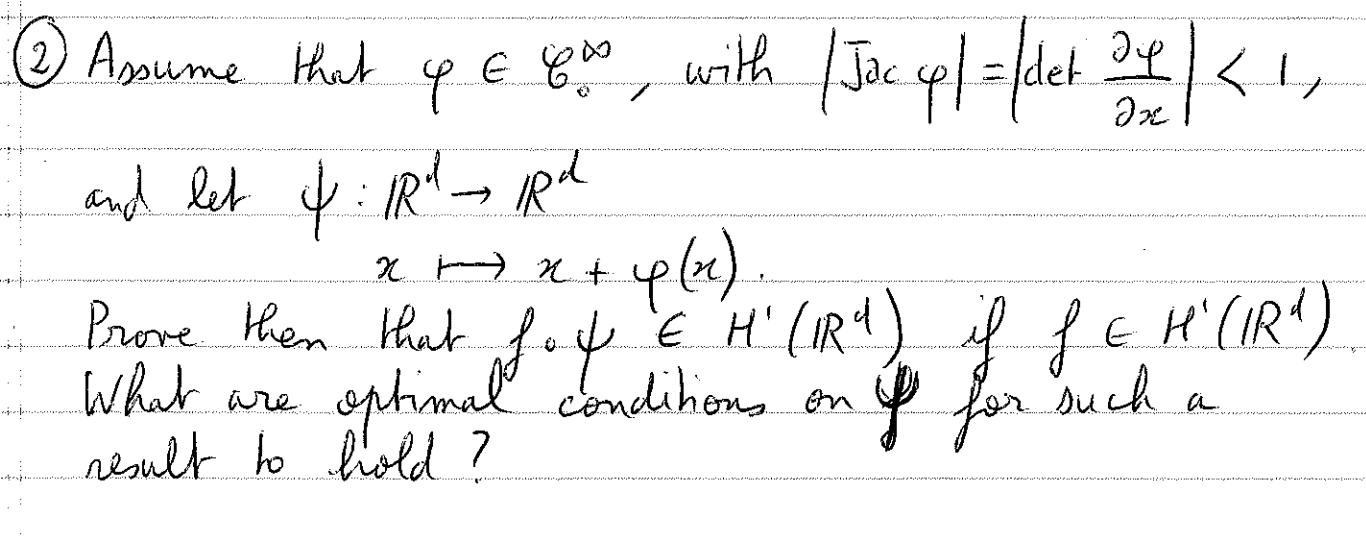
\includegraphics[width=0.7\textwidth]{pde2-s34-p2.png}
\end{figure}
\end{question}
\begin{solution} \hfill \\
As $|\text{det}\dfrac{\partial \phi}{\partial x}| < 1$, 
\eQb
||\partial_i(f \circ \psi)||_{L^2}^{2} &=& \int_{\mathbb{R}^d} 
|\triangle f|^2 + |\triangle f \cdot \dfrac{\partial \phi}{\partial x_i}|^2 dx 
\leq C||\triangle f||_{L^2}^{2}.
\eQe
Let $y = \Psi(x)$, and $\inf |\det \dfrac{\partial \Psi}{\partial x}| > 0$. Then,
by inverse function theorem, we have $h$ such that $\sup|\det h(y)|<\infty$,
and $h(y) = (D\Psi)^{-1}(y)$. Then, 
\eQb
\int_{\mathbb{R}^d} |f \circ \Psi(x)|^2 dx \leq \sup |\det h(y)| ||f||_{L^2}^{2} <
\infty.
\eQe
Now, consider $d \geq 3$, $f(x) = |x|^{\alpha}X(x)$, $X(x) \in C_{0}^{\infty}(
\mathbb{R}^d)$, $X = 1$ on $B(0,1)$, $\alpha > 1 - \dfrac{d}{2}$. We from
hw1 that $f \in H^1(\mathbb{R}^d)$. Now, set $\Psi(x) = |x|^2 x$ if $|x| < \dfrac{1}{2}
$ and $x$ if $|x| > 1$. Then, we see $f \circ \Psi \not\in H^1(\mathbb{R}^d)$ 
is equivalent $\alpha \geq \dfrac{1}{3} - \dfrac{d}{6}$. As $\alpha$
can be chosen to be in $(1-\dfrac{d}{2}, \dfrac{1}{3} - \dfrac{d}{6}]$, we see
that the condition is optimal. \hfill $\qed$

\end{solution}

\newpage

\begin{question}[1-3]
\hfill
\begin{figure}[h!]
  \centering
    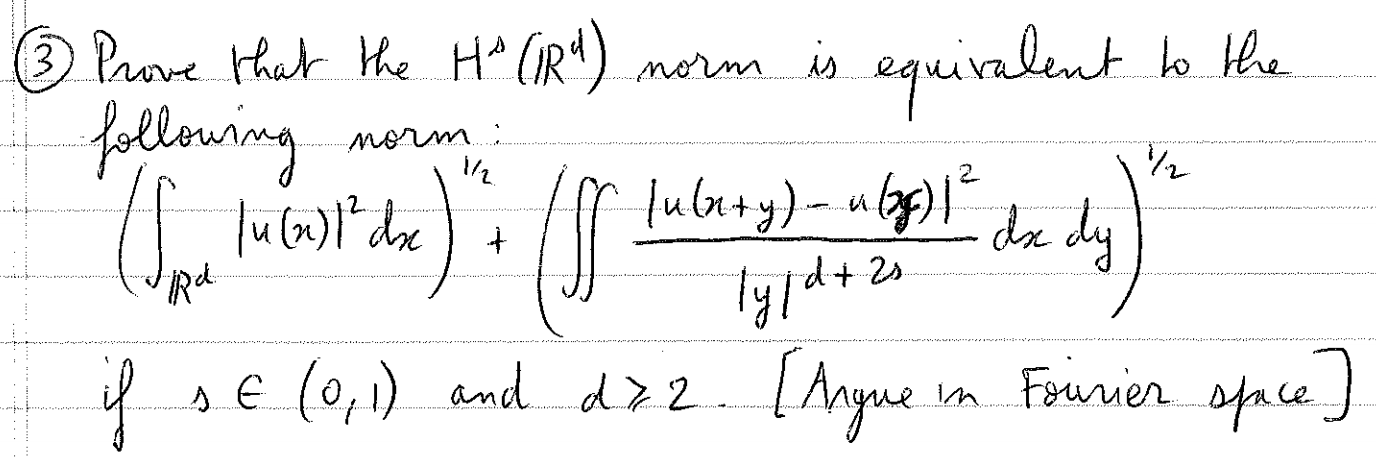
\includegraphics[width=0.7\textwidth]{pde2-s34-p3.png}
\end{figure}
\end{question}
\begin{solution} \hfill \\
We compute
\eQb
\int_{\mathbb{R}^d} \dfrac{|e^{iy\xi} - 1|^2}{|y|^{d+2s}} dy 
&\leq& C \left( \int_{|y| < \frac{1}{|\xi|}} \dfrac{|y|^2 |\xi|^2}{|y|^{d+2s}} dy 
+ \int_{|y| > \frac{1}{|\xi|}} \dfrac{1}{|y|^{d+2s}} dy \right) \\
&=& C \left( |\xi|^2 \int_{0}^{\frac{1}{|\xi|}} r^{- d - 2s + 2} r^{d-1} dr 
+ \int_{\frac{1}{|\xi|}}^{\infty} r^{-d-2s+d-1} dr \right) \\
&=& C\left( |\xi|^2 r^{-2s+2} \rvert_{0}^{\frac{1}{|\xi|}} + r^{2s} \rvert_{
\frac{1}{|\xi|}}^{\infty} \right) \sim <\xi>^{2s}.  
\eQe
Similarly, 
\eQb
\int_{\mathbb{R}^d} \dfrac{|e^{iy\xi} - 1|^2}{|y|^{d+2s}} dy \geq C|\xi|^{2s} 
\sim <\xi>^{2s}.
\eQe
Since, by Fubini,
\eQb
\int\int \dfrac{|u(x+y) - u(x)|^2}{|y|^{d+2s}} dx dy &=&
\int\int |e^{iy\xi} -1|^2 |\hat{u}(\xi)|^2 d\xi \dfrac{1}{|y|^{d+2s}} dy \\ 
&=& \int\int |e^{iy\xi} - 1|^2 \dfrac{1}{|y|^{d+2s}} dy |\hat{u}(\xi)|^2 d\xi,
\eQe
and the established asymtotics, we see the norm equivalence. \hfill $\qed$

\end{solution}

\newpage

\begin{question}[1-4]
\hfill
\begin{figure}[h!]
  \centering
    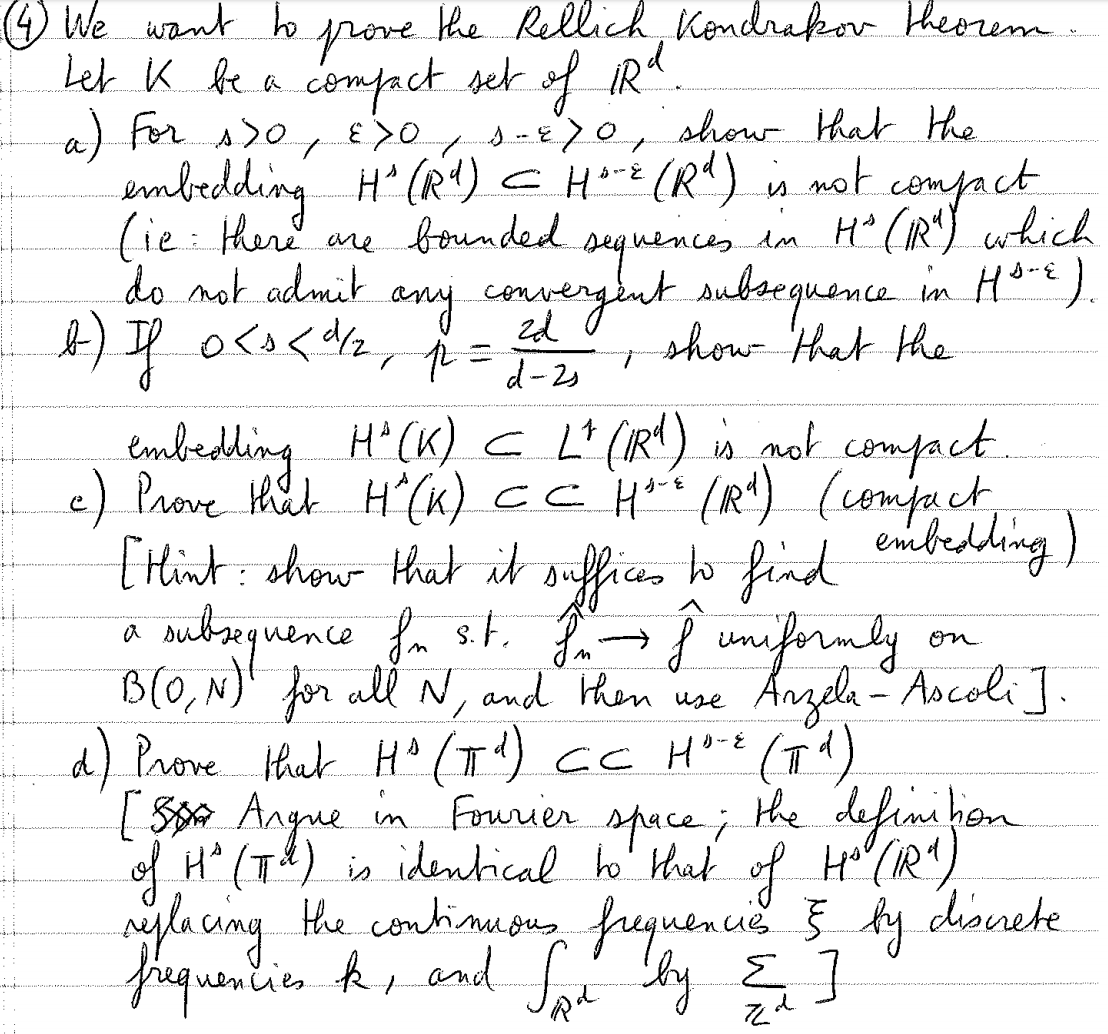
\includegraphics[width=0.7\textwidth]{pde2-s34-p4.png}
\end{figure}
\end{question}
\begin{solution} \hfill \\
\textbf{(a)} Let $B_n = B(0,\dfrac{1}{n})$, for $n \in \mathbb{N}$,
$\Omega_1 = B_1$, and $\Omega_n = B_n \setminus B_{n-1}$ for $n \geq 2$. Furthermore,
for each $n \in \mathbb{N}$, let 
\eQb
c_n &=& {\left(\int_{\Omega_n} <\xi>^{2s - 2\epsilon} d\xi \right)}^{-\frac{1}{2}} 
\>\>\> \text{and} \>\>\> \hat{f_n} = c_n 1_{\Omega_n}. 
\eQe 
Then,
\eQb
||f_n||_{H^{s-\epsilon}(\mathbb{R^d})} &=& \left(
\int_{\mathbb{R}^d} (<\xi>^{s - \epsilon}
\hat{f}(\xi))^2 d\xi \right)^{\frac{1}{2}}  
= \left( \int_{\Omega_n} c_n^2 <\xi>^{2s - 2\epsilon} d\xi \right)^{\frac{1}{2}} = 1
\eQe
for any $n \in \mathbb{N}$, and 
\eQnb
<f_n, f_m >_{H^{s-\epsilon}(\mathbb{R}^d)} &=& \int_{\mathbb{R}_d} <\xi>^{2s -
2\epsilon} \hat{f_n}(\xi) \hat{f_m}(\xi) d\xi = 0  \label{eq:1-4-1}
\eQne
for any $n,m \in \mathbb{N}$ with $n \neq m$, where~\eqref{eq:1-4-1} follows from 
the fact that $\hat{f_n}$ and $\hat{f_m}$ have disjoint supports, if $n \neq m$. 
Therefore,
\eQb
||f_n - f_m||_{H^{s-\epsilon}(\mathbb{R}^d)}^2 &=& <f_n - f_m, f_n - f_m> \\ 
&=& ||f_n||_{H^{s-\epsilon}(\mathbb{R}^d)}^2 + ||f_m||_{H^{s-\epsilon}(\mathbb{R}^d)}^2
- 2<f_n,f_m> = 2  
\eQe 
for any $n,m \in \mathbb{N}$, with $n \neq m$, so $\{f_n\}$ does not have a 
convergent subsequence in $H^{s-\epsilon}(\mathbb{R}^d)$. Furthermore, 
\eQnb
||f_n||_{H^{s}(\mathbb{R}^d)} = \int_{\Omega_n} {c_n}^2 <\xi>^{2s} d\xi = 
c_n^2 \int_{\Omega_n} {c_n}^2 <\xi>^{2s} d\xi \leq 2^{\epsilon} c_n^2
\int_{\Omega_N} <\xi>^{2s - 2\epsilon} d\xi = 2^{\epsilon} \label{eq:1-4-2} 
\eQne
for any $n \in \mathbb{N}$, where~\eqref{eq:1-4-2} holds by $<\xi> \leq 2$ for 
any $\xi \in B(0,1)$. Therefore, the embedding is not compact. 

\bigskip

\noindent \textbf{(b)} Let $f \in H^s(K)$ such that $||f||_{H^s} > 0$, 
and set $f_n = n^{\frac{d}{p}} f(n\cdot)$ 
for any $n  \in \mathbb{N}$. Then, $||f_n||_{L^p} = ||f||_{L^p}$ for all $n$,
and $f_n \to 0$ almost everywhere. We 
see that $\{f_n\}$ does not have any convergence subsequence, as if some $\{ f_{n_k}\}$
converges to some $g$ in $L^p$, then there is a further subsequence that convergence
to $g$, so $g = 0$, which is a contradiction, as $||g||_{L^p} = ||f||_{L^p} \geq 
||f||_{H^s(K)} > 0$, by continuity of the norm. Now,
\eQb
||f_n||_{H^s(K)}^2 &=& \int < \xi>^{2s} n^{2d(\frac{1}{p} - 1)} |f(\dfrac{\xi}{n})|^2
d\xi \\ 
&\leq& n^{2d(\frac{1}{p} - \frac{1}{2}) + 2s} \int (1+|\xi|^2)^{s} 
|\hat{f}(\xi)|^2 d\xi \\
&=& ||f||_{H_s(K)}^2 \\
\eQe
for all $n$, so we see that the inclusion is not compact. 

\bigskip

\noindent \textbf{(c)} Let $\{f_n\}$ be a sequence in $H^s(K)$ such that 
there exists a constant $C$ such that $||f_n||_{H^s(K)} \leq C$ for all $n \in 
\mathbb{N}$. Then,
\eQb
|\hat{f_n}(\xi + \delta) - \hat{f_n}(\xi)| &\le& `
\eQe

\bigskip

\noindent \textbf{(d)} 

\end{solution}
\end{document}

